\documentclass[10pt]{siamltex}
\usepackage[]{amsmath,amssymb,epsfig}
\usepackage[top=18mm, bottom=18mm, left=20mm, right=20mm]{geometry}

\usepackage{hyperref}
\usepackage{booktabs}
\usepackage{tabularx}
\usepackage{graphicx}
\usepackage[space]{grffile}
\usepackage{adjustbox}
\usepackage{verbatimbox}

\newcommand{\mb}[1]{\mbox{\boldmath$#1$}}

\usepackage{lineno}

\usepackage{subfigure}
\usepackage{amsmath}
\usepackage{amssymb}
\usepackage{graphicx}
\usepackage{comment}
\usepackage{array}
\usepackage{algorithm}
\usepackage{algorithmicx}
\usepackage{url}

\usepackage{setspace}
\usepackage{multicol}
\usepackage{multirow}
\usepackage{color}
\usepackage{colortbl}
\usepackage{xcolor}
\usepackage{hyperref}

\newcommand{\myreferences}{../../../Postdocs_laptop/postdoc_bib_file}

\hypersetup{
    colorlinks=true,
    citecolor=red,
    linkcolor=blue,
    urlcolor=blue
  }
  
\usepackage{listings}
\usepackage{color}

\definecolor{dkgreen}{rgb}{0,0.2,0}
\definecolor{gray}{rgb}{0.5,0.5,0.5}
\definecolor{mauve}{rgb}{0.58,0,0.82}

\lstset{frame=tb,
  language=R,
  aboveskip=3mm,
  belowskip=3mm,
  showstringspaces=false,
  columns=flexible,
  basicstyle={\small\ttfamily},
  numbers=none,
  numberstyle=\tiny\color{mauve},
  keywordstyle=\color{blue},
  commentstyle=\color{dkgreen},
  stringstyle=\color{mauve},
  breaklines=true,
  breakatwhitespace=true,
  tabsize=3
}

\newcounter{ale}
\newcommand{\abc}{\item[\alph{ale})]\stepcounter{ale}}
\newenvironment{liste}{\begin{itemize}}{\end{itemize}}
\newcommand{\aliste}{\begin{liste} \setcounter{ale}{1}}
\newcommand{\zliste}{\end{liste}}
\newenvironment{abcliste}{\aliste}{\zliste}



\begin{document}

\title{MATH 191 Topics in Data Science: \\ Algorithms and Mathematical Foundations \\ A comparison of correlation measures used for prediction of stock returns }
\author{Lawrence Ouyang}
\date{\today}
\maketitle

\begin{center}
     \today
\end{center}

\vspace{5mm}

\begin{abstract}
The prediction of the returns of a stock has been a very popular problem since the very existence of the stock market. Given the day's returns, what will tomorrow's look like? What will it look like next week, or next month? An idea to examine this is the use of correlation measures. The market is not an isolated system; all things affect one another. This work will use a variety of known correlation measures (Pearson's, Spearman's, Hoeffding, distance correlation) as a dimension reduction tool to compute the most relevant instruments to which we will apply linear regression. The goal is to find an accurate predictor for future returns. 
\end{abstract}


\begin{keywords} Correlation; Returns; Linear Regression
\end{keywords}


\section{Introduction}

The idea behind examining logarithmic returns is extremely rational. By using returns instead of raw prices, our values become normalized, which is a requirement for accurate comparisons and measurements. Logarithmic functions are log-normal as well, and as such, our returns our now normally distributed. However, with these benefits also come a price. The logarithmic returns does not have an implied one-to-one relationship with the simple returns, as well as having higher variance which can possibly reduce expected returns\cite{CompLogSimRet}. For simplicity, this paper will focus on the use of logarithmic returns to simplify our results. Below is a brief description of our correlation measures.

\subsection{Pearson Correlation}

The Pearson correlation is an extremely basic and simple correlation measure used for many statistical practices. It is defined as:

\begin{equation}
Cov(X,Y) = \sum_{i=1}^n\frac{(x_i - \bar{X})(y_i - \bar{Y})}{n-1}
\end{equation}
\begin{equation}
Cor(X,Y) = \frac{Cov(X,Y)}{Var(X)Var(Y)}
\end{equation}
 However, because of it's simplicity, the Pearson correlation faces many shortcomings. As shown in equation 1.1, the covariance is greatly affected if $x_i, y_i$ are extremely large or small values. Since Pearson only measure linear relationships, any nonlinear dependency will not be represented\cite{CorComp}. 

\subsection{Spearman's Rank Correlation}

Spearman's correlation is similar to Pearson's except rather than using raw values, Spearman uses ranked values. This better normalizes the data set and accounts for extreme values in the correlation. Consider $d$ to be the distance between rank $x_i, y_i$, then Spearman's rank correlation can be calculated as\cite{CompGeneExpress}:

\begin{equation}
\rho_{Spearman}(X,Y) = 1 - \frac{6\sum_{i=1}^nd_i^2}{n(n^2 - 1)}
\end{equation}

Spearman also suffers the same shortcomings as Pearson, however, it does handle certain cases more gracefully, and thus is often also considered alongside Pearson.

\subsection{Hoeffding's D}

Determining our significant predictors using only a standard correlation measure like Pearson or Spearman would be too mundane. We instead examine other measurements, beginning with Hoeffding's D.
Hoeffding's D measures the difference of joint ranks and the product of the marginal ranks. The shortcomings of Spearman and Pearson are their inability to detect nonlinear relationships. However, Hoeffding's D is capable of this, making it more versatile\cite{CorComp}.

\subsection{Distance Correlation}

The distance correlation simply uses the euclidean distance between our data points to calculate the correlation\cite{CorDist}. Similar to Hoeffding's D, distance correlation is able to identify nonlinear relationships, making it more versatile. It is also relatively easy to implement. Consider the distant covariance:
\begin{equation}
dCov(X,Y) = \sqrt{\frac{1}{n^2}\sum_{i,j=1}^nx_{ij}y_{ij}}
\end{equation}
\begin{equation}
dVar(X) = dCov(X,X) \hspace{8mm} dVar(Y) = dCov(Y,Y)
\end{equation}
\begin{equation}
dCor(X,Y) = \frac{dCov(X,Y)}{\sqrt{dVar(X)dVar(Y)}}
\end{equation}

With the above measurements considered, in Section \ref{sec:ourWork} we put them to the test by extracting the top values and using it for linear regression. 
In Section \ref{sec:NumExpReal} we test the algorithms for a real data set. Finally, in Section  \ref{sec:conclusion} we conclude with a summary of our results, and discuss future possible research direction. 

\vspace{5mm}

\section{Related work} \label{sec:relWork}

\begin{center}
	\textit{Some questions that should be considered before continuing.}
\end{center}

\vspace{2mm}

\begin{itemize}
\item Since obtaining such large correlation matrices are calculation intensive, what other methods can be used to trim our selection before creating our matrices?
\item What kind of accuracy would using the correlation of alternating entries give? 
\item Which correlation measure is most affective, and why?
\item How many instruments should be considered when building our model? Using more would increase our R-squared, but would it result in over-fitting?
\item Disregarding computing time, how much data should be used to build the correlation matrices?
\end{itemize}

\vspace{5mm}

\section{Our work}    \label{sec:ourWork}
\subsection{The Data}

The data set being used is the logarithmic return prices from date to date for 477 stocks. Since the data contains many not-available entries, we begin by stripping those out of our measurements. Instruments with a high number of NA entries are entirely removed along with missing rows. This leaves us with a dataset containing 436 instruments with data for 2629 days. This presents a problem: our dataset is too large to due a correlation function in a reasonable time frame. To combat this, we will only use the first 500 entries to determine correlation. The remaining values will be used to as our test matrix.

\subsection{The Process}
With our primmed and proper data, we begin by calculating their coefficient matrices. Considering the size of our data, the calculation of our coefficient matrices take a very large amount of time. 
Of course, building the matrices is the simple, although lengthy, part. \vspace{5mm}\\
Now for the instrument we would like to predict, we need to sort it's correlation values in descending order and choose the amount to use in our linear regression. Once sorted, we build our linear regression model and evaluate its accuracy.\vspace{5mm} \\
With our model, we then use our remaining data points to create a predicted vector $\hat{y}$. We then compare our prediction with the actual values, and calculate the average error $\epsilon$.$\epsilon$ is defined as:
\begin{equation}
\epsilon = |\frac{y - \hat{y}}{nrow - 100}|
\end{equation}
We want a minimized error $\epsilon$ as that would denote a more accurate prediction. Our results are shown in the next section.
\newpage
\section{Numerical Results}   \label{sec:NumExpReal}
The tables below represents a selection of 5 instruments, and the 20 instruments that had the strongest relationships from left to right with them. This includes the average error and the adjusted R-squared value for the given regression model.\\
\begin{center} \label{tab:relation}
Pearson \\
\begin{adjustbox}{width = 1\textwidth}
	\small
\addvbuffer[10pt 5pt]{\begin{tabular}{c|cccccccccccccccccccc}\toprule[1.5px]
	\textbf{SPY} & C & JPM & GS & AXP & MS & GE & BBT & TROW & WFC & KEY & EMR & NTRS & PPG & ITW & ETN & LNC & PCAR & BEN & BK & CINF\\
	\midrule
	\textbf{YHOO} & AMZN & EBAY & SPY & NTAP & LLTC & ADI & VRSN & XLNX & JBL & KLAC & TER & JDSU & MOLX & JNPR & AMAT & FISV & BRCM & TMO & LRCX & ADBE \\
	\midrule
	\textbf{DELL} & SPY & LLTC & CSCO & INTC & ADI & AMAT & MOLX & XLNX & MSFT & KLAC & CTAS & ALTR & IBM & PCAR & LRCX & TXN & HPQ & JBL & PBI & AXP \\
	\midrule
	\textbf{AAPL} & SPY & IR & NTAP & PPG & INTC & CSCO & LLTC & MSFT & JCI & DELL & JNPR & SIAL & PCAR & CHRW & PH & PBI & YHOO & FISV & AA & ITW \\
	\midrule
	\textbf{IBM} & SPY & MSFT & LLTC & AXP & INTC & MS & OMC & XLNX & AMAT & CSCO & C & MOLX & BK & ORCL & GS & PCAR & SCHW & TROW & ADI & CINF\\
	\bottomrule[1.25px]
\end{tabular}}
\end{adjustbox} \\ 
	\addvbuffer[5pt 20pt]{\begin{tabular}{cccccc}\toprule[1.5px]
		& \textbf{SPY} & \textbf{YHOO} & \textbf{DELL} & \textbf{AAPL} & \textbf{IBM} \\
		\midrule
		R-Squared & 0.8825 & 0.5807 & 0.4723 & 0.2501& 0.5363\\
		\midrule
		Error $\epsilon$ & 0.00414 & 0.01414 & 0.01117& 0.01454& 0.00656\\
		\bottomrule[1.25px]
	\end{tabular}} \\
Spearman \\
\begin{adjustbox}{width = 1\textwidth}
	\small
	\addvbuffer[10pt 5pt]{\begin{tabular}{c|cccccccccccccccccccc}\toprule[1.5px]
			SPY & C & AXP & GS & JPM & NTRS & MS & STI & ETN & PCAR & BBT & BEN & TROW & DOV & GE & WFC & EMR & KEY & LM & LNC & BAC \\
			\midrule
			YHOO & EBAY & AMZN & SPY & NTAP & JNPR & VRSN & JDSU & ADI & XLNX & LLTC & TER & JBL & KLAC & ADBE & TXN & INTC & BRCM & QCOM & FFIV & MOLX \\
			\midrule
			DELL & SPY & INTC & CSCO & LLTC & AMAT & MSFT & ADI & LRCX & IBM & XLNX & CTAS & PCAR & HPQ & NTAP & MOLX & ALTR & ORCL & KLAC & TXN & BRCM \\
			\midrule
			AAPL & SPY & NTAP & INTC & JNPR & DELL & MSFT & IR & CSCO & BRCM & PCAR & PPG & SIAL & DOV & LLTC & FISV & JCI & PH & CHRW & MOLX & ORCL \\
			\midrule
			IBM & SPY & MSFT & INTC & CSCO & C & XLNX & DELL & ORCL & LLTC & CTAS & ADBE & MS & AXP & FISV & SCHW & OMC & PCAR & AMAT & CINF & LM \\
			\bottomrule[1.25px]
		\end{tabular}}
	\end{adjustbox}
	\addvbuffer[5pt 20pt]{\begin{tabular}{cccccc}\toprule[1.5px]
			& \textbf{SPY} & \textbf{YHOO} & \textbf{DELL} & \textbf{AAPL} & \textbf{IBM} \\
			\midrule
			R-Squared & 0.8851 & 0.5780 & 0.4741 & 0.2514& 0.5365\\
			\midrule
			Error $\epsilon$ & 0.00469 & 0.01422 & 0.01118& 0.01447& 0.00658\\
			\bottomrule[1.25px]
		\end{tabular}} \\
Hoeffding's D \\
\begin{adjustbox}{width = 1\textwidth}
	\small
	\addvbuffer[10pt 5pt]{\begin{tabular}{c|cccccccccccccccccccc}\toprule[1.5px]
			SPY & C & AXP & NTRS & JPM & GS & MS & BEN & PCAR & DOV & ETN & STI & BBT & TROW & GE & KEY & LM & WFC & MLX & LNC & EMR \\
			\midrule
			YHOO & EBAY & AMZN & SPY & NTAP & VRSN & TER & JNPR & XLNX & JDSU & LLTC & JBL & ADI & KLAC & QCOM & ADBE & TXN & FFIV & INTC & AMAT & ROP \\
			\midrule
			DELL & SPY & INTC & CSCO & LLTC & MSFT & AMAT & IBM & ADI & LRCX & HPQ & MOLX & XLNX & TAS & ORCL & ALTR & BRCM & NTAP & PCAR & JDSU & TXN \\
			\midrule
			AAPL & SPY & NTAP & INTC & DELL & JNPR & MSFT & IR & BRCM & PCAR & CSCO & ORCL & DOV & MOLX & SIAL &LLTC & CTAS & PPG & CHRW & FSIV & JCI \\
			\midrule
			IBM & SPY & MSFT & INTC & CSCO & FISV & C & DELL & ORCL & ADBE & XLNX & AXP & LLTC & CTAS & OMC & HPQ & MOLX & HIG & CSC & PCAR & AMAT \\
			\bottomrule[1.25px]
		\end{tabular}}
	\end{adjustbox}
	\addvbuffer[5pt 20pt]{\begin{tabular}{cccccc}\toprule[1.5px]
			& \textbf{SPY} & \textbf{YHOO} & \textbf{DELL} & \textbf{AAPL} & \textbf{IBM} \\
			\midrule
			R-Squared & 0.8937 & 0.5793 & 0.4756 & 0.2515& 0.5432\\
			\midrule
			Error $\epsilon$ & 0.00444 & 0.01423 & 0.0112& 0.01450& 0.00673\\
			\bottomrule[1.25px]
		\end{tabular}} \\
Distance\\
\begin{adjustbox}{width = 1\textwidth}
	\small
	\addvbuffer[10pt 5pt]{\begin{tabular}{c|cccccccccccccccccccc}\toprule[1.5px]
			SPY & C & JPM & GS & AXP & NTRS & MS & BBT & STI & TROW & PCAR & ETN & DOV & BEN & GE & KEY & WFC & EMR & LM & BAC & LNC \\
			\midrule
			YHOO & EBAY & AMZN & SPY & NTAP & VRSN & JNPR & TER & ADI & XLNX & JDSU & LLTC & JBL & KLAC & ADBE & TXN & INTC & BRCM & A & FFIV & QCOM \\
			\midrule
			DELL & SPY & INTC & CSCO & LLTC & AMAT & MSFT & ADI & LRCX & IBM & XLNX & CTAS & MOLX & HPQ & ALTR & PCAR & KLAC & NTAP & ORCL & TXN & BRCM \\
			\midrule
			AAPL & SPY & NTAP & INTC & JNPR & DELL & MSFT & IR & CSCO & BRCM & PCAR & PPG & SIAL & LLTC & DOV & MOLX & FISV & JCI & ORCL & YHOO & CTAS \\
			\midrule
			IBM & SPY & MSFT & INTC & CSCO &C & XLNX & LLTC & AXP & OMC & CTAS & ORCL & MS & DELL & FISV & ADBE & AMAT & SCHW & PCAR & MOLX & BK \\
			\bottomrule[1.25px]
		\end{tabular}}
	\end{adjustbox}
	\addvbuffer[5pt 20pt]{\begin{tabular}{cccccc}\toprule[1.5px]
			& \textbf{SPY} & \textbf{YHOO} & \textbf{DELL} & \textbf{AAPL} & \textbf{IBM} \\
			\midrule
			R-Squared & 0.8851 & 0.5778 & 0.4741 & 0.2447& 0.5358\\
			\midrule
			Error $\epsilon$ & 0.00607 & 0.01534 & 0.01231& 0.0137& 0.00702\\
			\bottomrule[1.25px]
		\end{tabular}} \\

\end{center}
\newpage
\vspace*{\fill}
\begin{figure}[h]
	\begin{center}
		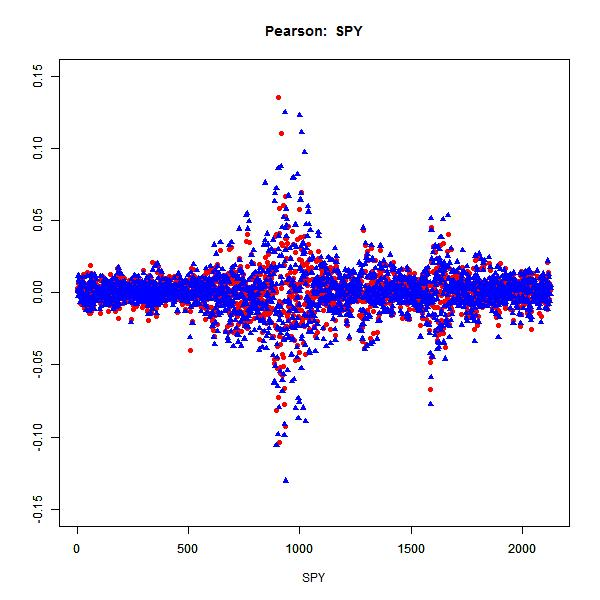
\includegraphics[width=0.46\columnwidth]{Images/PearsonSPY}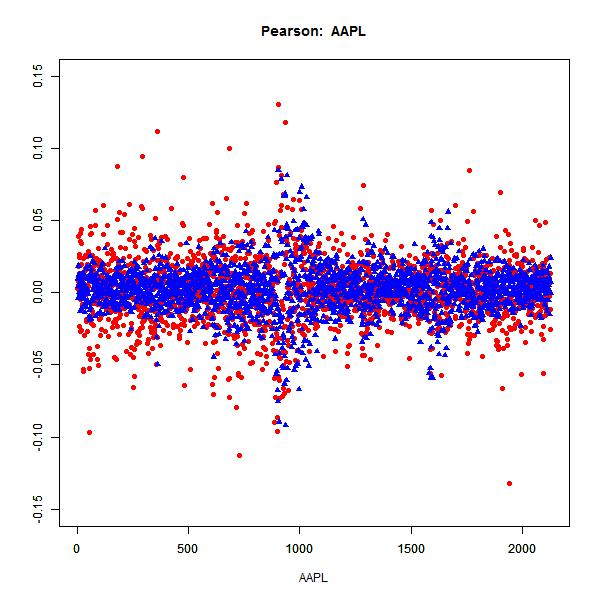
\includegraphics[width=0.46\columnwidth]{Images/PearsonAAPL}\\
		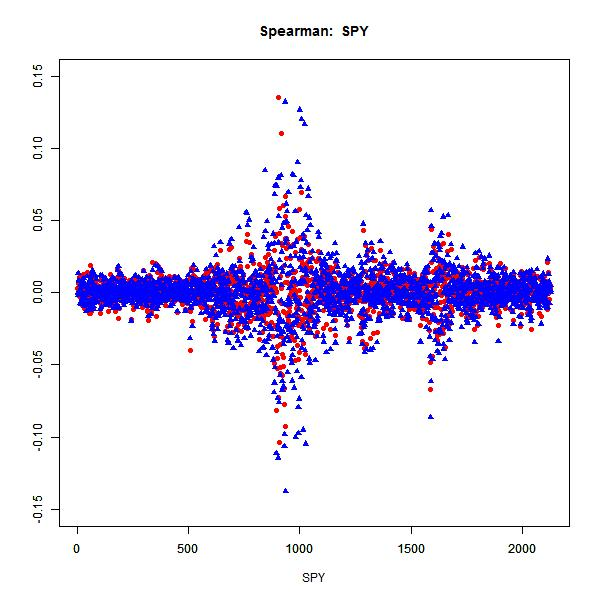
\includegraphics[width=0.46\columnwidth]{Images/SpearmanSPY}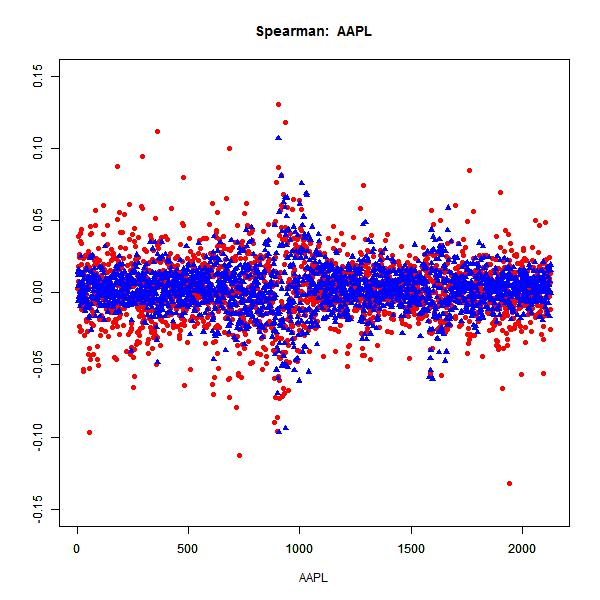
\includegraphics[width=0.46\columnwidth]{Images/SpearmanAAPL}
	\end{center}
	\caption{The scatterplot for our real values and prediction values of instrument \textit{SPY}. and \textit{AAPL} for Pearson and Spearman. Due to the density, it is difficult to see point by point the differences, but the relationship is still quite clear.}
	\label{fig:PearSpear}
\end{figure}
\vspace*{\fill}
\newpage
\vspace*{\fill}
\begin{figure}[h]
	\begin{center}
		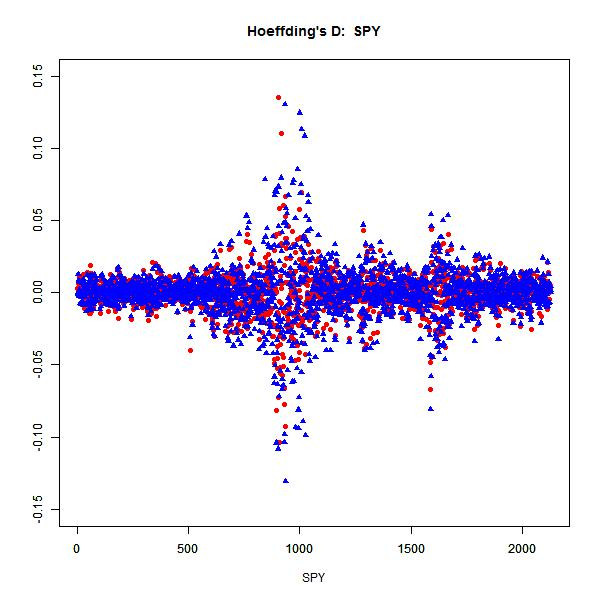
\includegraphics[width=0.46\columnwidth]{Images/HoeffdingSPY}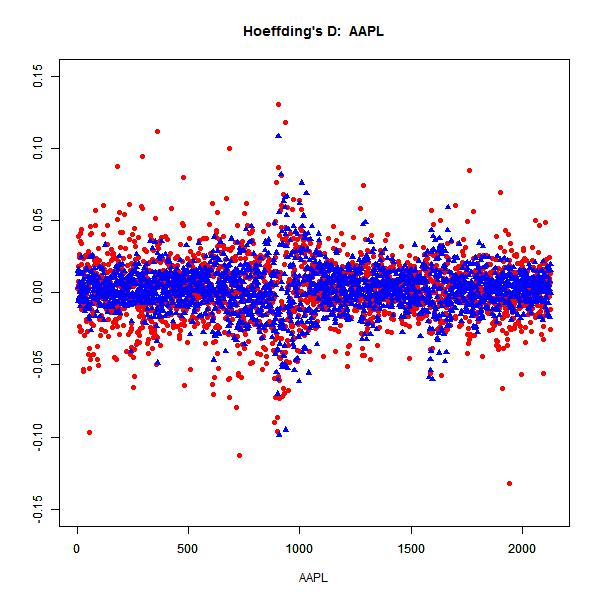
\includegraphics[width=0.46\columnwidth]{Images/HoeffdingAAPL}\\
		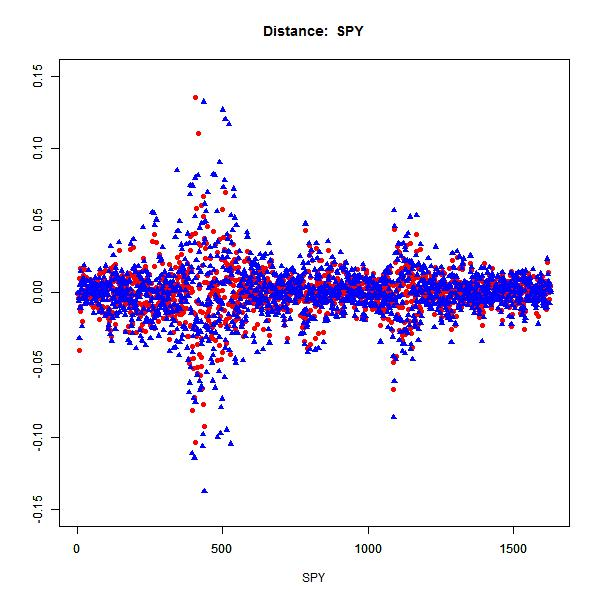
\includegraphics[width=0.46\columnwidth]{Images/DistanceSPY}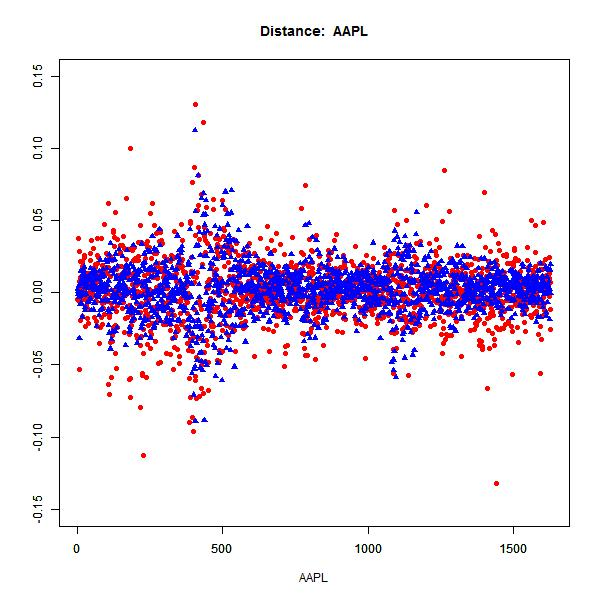
\includegraphics[width=0.46\columnwidth]{Images/DistanceAAPL}\\
	\end{center}
	\caption{The The scatterplot for our real values and prediction values of instrument \textit{SPY}. and \textit{AAPL} for Hoeffding's D and distance correlation.  Due to the density, it is difficult to see point by point the differences, but the relationship is still quite clear.}
	\label{fig:HoeffDist}
\end{figure}
\vspace*{\fill}
\newpage


\section{Results}  \label{sec:conclusion}

\subsection{Summary}

 We can easily note that \textit{SPY} has strong relationships with the other instruments. Other big industry names arise as well, with \textit{AMZN}, \textit{DELL}, \textit{IBM}, \textit{JNPR}, and \textit{AXP} appear quite often. This probably indicates that their presence greatly affects the economy of even smaller industries. Examining the tables in \ref{tab:relation}, we see that the different correlation produce very similar rankings, which is the reason why our results are very similar.  \vspace{2mm} \\
As expected, we see no clear results from our Pearson and Spearman models. They seem to show varying results. Hoeffding's D and distance correlation do not give much exciting results either, mirroring very closely to Pearson and Spearman. Hoeffding's D does have slightly lower error values than the standard, which may indicate a more viable prediction, while distance correlation gives less accurate results. Figure \ref{fig:HoeffDist} agrees with our result. More information can be found by repeated testing with all 477 instruments. We do note that instruments with strong relationships, such as \textit{SPY}, have high R-squared values and low errors. This may demonstrate that correlation ranking models are effective only on predicting major stock returns. Intuitively, since stronger relationships like with \textit{SPY} greatly affect other instruments, we can reasonably assume that it takes closer form to a linear relationship with overall increases or decreases based on other instruments. Weaker instruments will thus take a more nonlinear form, as a large number of less strong correlations can result in nonlinearity. This perhaps can be tested using other regression models.

\subsection{Conclusion}
Although not perfect, our correlation ranking selection method does produce a model with a degree of good accuracy, but only for select instruments. Distance correlation, unfortunately, seems inefficient as the calculations required to compute the correlation matrix is extremely high. The results of Pearson, Spearman, and Hoeffding's D are relatively similar for our chosen instruments. Since these 3 correlation measures are relatively simple to compute, all three can be used when analyzing strong relationship instruments such as \textit{SPY}.  Using this model, it is very possible to create an investment method such that we have improved Sharpe ratios. Although more testing is required, these results do demonstrate why correlation is such a prevalent statistical tool. 

\bibliographystyle{siam}
\bibliography{project_math191}

\end{document}



